\chapter{Iridis Oops!} 
\label{sec:bugs}
\lstset{style=6502Style}

\section{The Byte that Broke}
\begin{definition}[Jeffrey Says]
\setlength{\intextsep}{0pt}%
\setlength{\columnsep}{3pt}%
\begin{wrapfigure}{l}{0.12\textwidth}
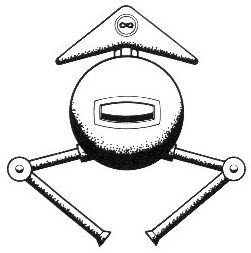
\includegraphics[width=\linewidth]{src/callout/ia.jpg} 
\end{wrapfigure}
\small
We must apologise to some of the earliest purchasers of IA, as well... it
seems that some data was corrupted during the production phase of the
data duplication, and the first few hundred copies of the game used to bug
out if you lost at the Bonus Phase All the buggy copies known of have
been replaced, and all current tapes are fine, but if you find you have a
buggy version you should send it back to those awfully nice Hewsons
people and they ll give you an unglitchified one,
\end{definition}

What happened is that the master tape had dropped the very last byte in the second
section of game data on the tape.

\begin{figure}[H]
  {
    \begin{adjustbox}{width=10cm,center}
      \surface{bugs/spool-sections-glitches.png}
    \end{adjustbox}
  }\caption[]{The problematic section of data highlighted in red.}
\end{figure}

\begin{figure}[H]
  {
    \setlength{\tabcolsep}{3.0pt}
    \setlength\cmidrulewidth{\heavyrulewidth} % Make cmidrule = 
    \begin{adjustbox}{width=5cm,center}

      \begin{tabular}{rllllllll}
        \toprule
        Start Address & End Address & Note & \\
        \toprule
\icode{0800} & \icode{BFFE}  & .\\
\icode{BF00} & \icode{BFFF}  & .\\
\icode{C000} & \icode{CFFE}  & .\\
\icode{E000} & \icode{F7FF}  & .\\
        \addlinespace
        \bottomrule
      \end{tabular}

    \end{adjustbox}

  }\caption{Chunk \icode{BF00} is missing its last byte.}
\end{figure}

\begin{lstlisting}[caption=The data segment as it should be\, with \icode{\$A2} at \icode{\$BFFF},escapechar=\%]
$BFFF	A2 07       LDX #$07
$C001	A9 08       LDA #$08
$C003	8D F8 BF    STA $BFF8
\end{lstlisting}

\begin{lstlisting}[caption=The corrupt byte\, with \icode{\$00} at \icode{\$BFFF},escapechar=\%]
$BFFF 00          BRK
$C000 07 A9       SLO $A9
$C002 08          PHP
$C003	8D F8 BF	  STA $BFF8
\end{lstlisting}

\section{Reappearing Enemies}

When you start a new game, enemies\index{enemies} from the previous game show up in the first
wave. For most people starting out, this will take the form of a few residual
'licker ships' zapping them just as they're getting started.

This bug happens because the 'wave' data isn't cleared down when a new game
starts. So whatever is in there from the previous game gets used until they're
flushed out by being killed and replaced with the level's proper enemy data.

This isn't a problem for the first game after Iridis Alpha is loaded because
the first level's data is hardcoded in there.

The fix is simple enough, we initialize the active wave data stored in `activeShipsWaveDataLoPtrArray\index{activeShipsWaveDataLoPtrArray}` and `activeShipsWaveDataHiPtrArray\index{activeShipsWaveDataHiPtrArray}`
with the first level's data whenever we start a new game. 

\begin{lstlisting}[caption=Fixing the reappearing enemy bug,escapechar=\%]
  LDA #$0F 
  STA $D418    ;Select Filter Mode and Volume 
  JSR ClearPlanetTextureCharsets%\index{ClearPlanetTextureCharsets}% 
  JSR InitializeActiveShipArray ; Added to fix the bug.
  JMP PrepareToLaunchIridisAlpha%\index{PrepareToLaunchIridisAlpha}% 

;------------------------------------------------------------------ 
; InitializeActiveShipArray 
;------------------------------------------------------------------ 
InitializeActiveShipArray 
  LDX #$00 
InitializeActiveShipLoop 
  LDA <planet1Level1Data%\index{planet1Level1Data}% 
  STA activeShipsWaveDataLoPtrArray%\index{activeShipsWaveDataLoPtrArray}%,X 
  LDA >planet1Level1Data%\index{planet1Level1Data}% 
  STA activeShipsWaveDataHiPtrArray%\index{activeShipsWaveDataHiPtrArray}%,X 
  INX 
  CPX #$10 
  BNE InitializeActiveShipLoop 
  RTS 
\end{lstlisting}

\section{A Sort of Cheat}

After a minute or two in the title screen\index{screen}, the game enters 'Attract Mode' and
plays a random level on autopilot for a few seconds. If you press F1 during
this play you enter the 'Made in France' pause-mode mini game. If you press F1
again you can now start playing the level 'Attract Mode' selected at random.

This is because the `CheckKeyboardInGame\index{CheckKeyboardInGame}` routine\index{routine} doesn't try to prevent you
from entering 'Pause Mode' while Attract Mode is running:

\begin{lstlisting}[caption=Fixing the reappearing enemy bug,escapechar=\%]
CheckKeyboardInGame%\index{CheckKeyboardInGame}%
        LDA lastKeyPressed%\index{lastKeyPressed}%
        CMP #$40 ; $40 means no key was pressed
        BNE KeyWasPressed%\index{KeyWasPressed}%
        LDA #$00
        STA f1WasPressed%\index{f1WasPressed}%
ReturnEarlyFromKeyboardCheck%\index{ReturnEarlyFromKeyboardCheck}%   
        RTS

KeyWasPressed%\index{KeyWasPressed}%   
        LDY f1WasPressed%\index{f1WasPressed}%
        BNE ReturnEarlyFromKeyboardCheck%\index{ReturnEarlyFromKeyboardCheck}%
        LDY attractModeCountdown%\index{attractModeCountdown}%
        BEQ b787C
        ; If a key is pressed during attract mode, accelerate the
        ; countdown%\index{countdown}% so that it exits it nearly immediately.
        LDY #$02
        STY attractModeCountdown%\index{attractModeCountdown}%
\end{lstlisting}

